\section{Grundlagen}

\subsection{Lerninhalt}
\begin{itemize}
   \item Sie kennen die Bezugsquellen und die verschiedenen Versionen von Linux
   \item Sie kennen den Aufbau des Source-Codes von Linux
   \item Sie kennen den Buildprozess des Linux-Kernels
   \item Sie kennen den modularen Aufbau von Linux
   \item Sie kennen die Code-Konventionen von Linux
   \item Sie kennen den Entwicklungsprozess von Linux
\end{itemize}

\subsection{Source-Code} \index{Linux-Kernel}


Der Source-Code des Linux-Kernels ist auf \url{https://www.kernel.org/} verfügbar.
Auf der Webseite werden verschiedene Versionen angeboten, die sich folgendermassen kategorisieren lassen:
\\

\begin{figure}[h!]
   \begin{center}
      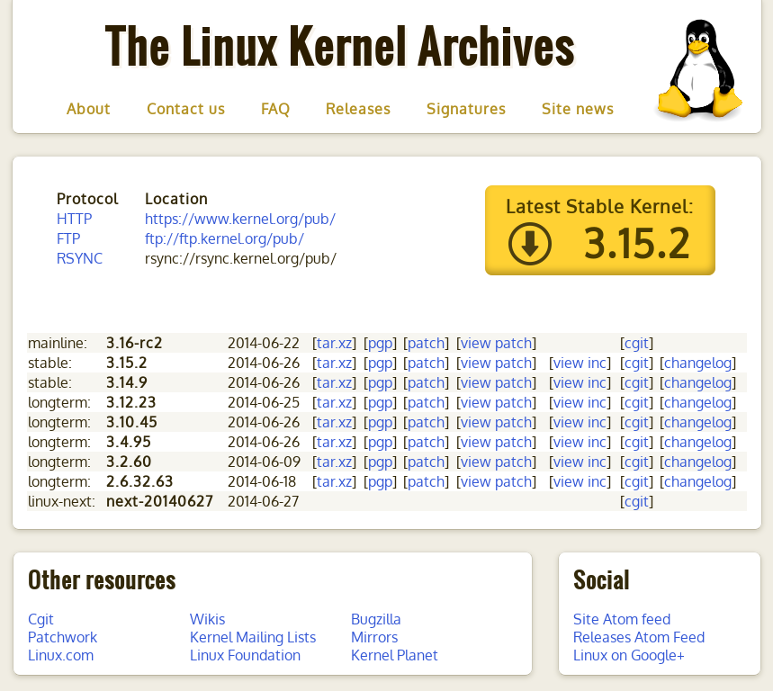
\includegraphics[scale=0.5]{images/kernel_org}
   \end{center}
   \caption[Kernel.org]{Linux-Kernel Webseite}
\end{figure}



\begin{description}
   \item[Mainline]
      Die Mainline entspricht der aktuellen Entwicklungsversion von Linus Torvalds\index{Linus Torvalds}. Alle von ihm
      abgesegneten Patches werden in diesen Tree\index{Tree} übernommen. Diese Version ist nicht für den produktiven
      Einsatz gedacht. Möchte man eigene Patches in den Linux-Kernel einbringen, so ist es jedoch Pflicht, diese 
      gegen die Mainline zu testen.

   \item[Stable]
      Alle zwei bis drei Monate gibt Linus Torvalds eine Mainline-Version als \emph{stable} frei. In diese Version fliessen 
      keine neuen Features mehr ein. Es werden nur noch Bugfixes von der Mainline übernommen und ist somit für den allgemeinen
      Gebrauch geeignet. Nach einer gewissen Zeit werden die stabilen Versionen als \emph{End of Life (EOL)}\index{End of Life (EOL)}
      bezeichnet. Ab diesem Zeitpunkt sollte auf eine neuere Version gewechselt werden.

   \item[Longterm]
      Kernel-Versionen, die von den grossen Linux-Distributionen\index{Linux-Distribution} verwendet werden, erhalten oft über mehrere
      Jahre Support. Diese werden als Longterm bezeichnet.
\end{description}


\subsection{Aufbau} \index{Source-Code}

Beim Arbeiten am Linux-Kernel ist es oft notwendig Funktions- und Strukturdefinitionen direkt im Source-Code nachzuschauen. Deshalb ist
es hilfreich zu wissen, wie der Source-Code aufgebaut ist. \hfill \\

\begin{minipage}{0.76\textwidth}
\begin{description}[leftmargin=3cm]
   \item[arch]
      Enthält den plattformspezifischen Code.
      Pro Architektur gibt es jeweils einen Unterordner (arm, i64, x86, etc.).

   \item[block]
      Implementation des Subsystems für blockorientierte Gerätetreiber.

   \item[crypto]
      Das Crypto-API bietet kryptographische Algorithmen für den Kernel an.
      Implementiert sind unter anderem SHA, Blowfish, Twofish, DES und AES. 

   \item[Documenation]
      Dieses Verzeichnis beinhaltet die Kernel-Dokumentation. Es ist eines der wichtigsten
      Werkzeuge um den Aufbau des Linux-Kernels zu verstehen.

   \item[drivers]
      Hier sind alle Treiber implementiert. Es ist mit Abstand das grösste Verzeichnis. Die Treiber
      sind jeweils nach den Subsystemen sortiert. Eine besondere Rolle nimmt \emph{staging} ein. Darin
      sind Treiber zusammengefasst, die noch instabil sind und erst in Zukunft integriert werden sollen. 

   \item[fs]
      Die Unterstützung von Filesystemen werden in diesem Verzeichnis implementiert. Diverse bekannte Formate, wie
      \emph{ext2}\index{ext2}, \emph{ext3}\index{ext3}, \emph{ext4}\index{ext4}, \emph{fat}\index{fat}, \emph{ntfs}\index{ntfs},
      \emph{nfs} und auch die virtuellen Formate wie \emph{proc}\index{proc}, \emph{sysfs}\index{sysfs} und \emph{debugfs}\index{debugfs} sind
      hier zu finden.
      
   \item[include]
      Eine Sammlung von C-Headern des Cores und den Subsystemen.

   \item[init]
      Die allgemeine Startroutine des Linux-Kernels, welche nach der plattformspezifischen Initialisierung aufgerufen wird.

   \item[ipc]
      Umsetzung der \emph{Inter-Process Communication (IPC)}\index{Inter-Process Communication (IPC)}. Beinhaltet \emph{Shared-Memory}\index{Shared-Memory},
      \emph{Semaphore}\index{Semaphore} und \emph{Message-Queues}\index{Message-Queue}.

   \item[kernel]
      Beinhaltet die Core-Funktionen wie das \emph{Scheduling}\index{Scheduling}, die \emph{Interrupthandler}\index{Interrupt} und die \emph{Locking-Mechanismen}\index{Locking}.
\end{description}
\end{minipage}
\hfill
\begin{minipage}{0.18\textwidth}
   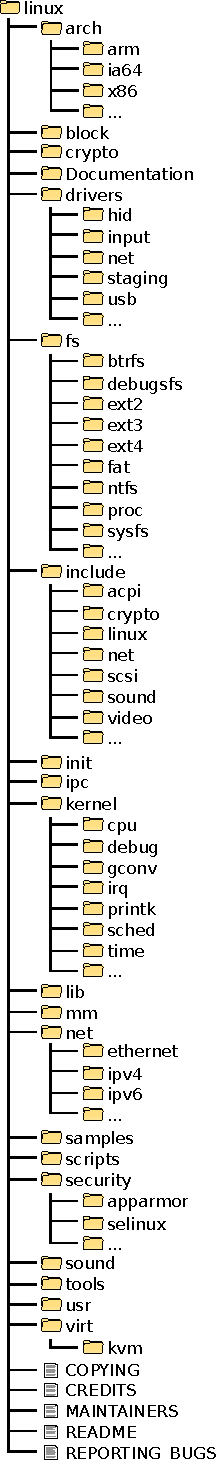
\includegraphics[width=\textwidth]{images/linux_source}
\end{minipage}

\begin{description}[leftmargin=3cm]

   \item[lib]
      Allgemeine Bibliotheksfunktion, zum Beispiel für die Stringmanipulation, sind unter diesem Verzeichnis zu finden.

   \item[mm]
      Das \emph{Memory-Mangement (MM)}\index{Memory-Management (MM)} ist für die Bereitstellung des \emph{virtuellen Speichers}\index{Virtueller Speicher} zuständig.


   \item[net]
      Der Netzwerk-Stack inklusive Protokollimplementationen für IPv4\index{IPv4}, IPv6\index{IPv6} und viele weitere sind hier zu finden.

   \item[samples]
      Eine Sammulung von Beispielcodes.

   \item[scripts]
      Diverse Scripts bilden eine Hilfestellung für die Kernel-Entwickler. 

   \item[security]
      Unter \emph{security} sind verschiedene optionale Sicherheitsframesworks zu finden. Die bekannsten sind \emph{SELinux}\index{SELinux}
      und das in Ubuntu standardmässig aktivierte \emph{AppArmor}\index{AppArmor}.

   \item[sound]
      Implementiert den Audio-Stack.

   \item[tools]
      Userspace-Werkzeuge\index{Userspace}, die von den Kernel-Entwicklern gepflegt werden, sind hier untergebracht.

   \item[usr]
      Buildfunktionen für das Erstellen des Linux-Image.

   \item[virt]
      Virtualisierungslösungen, welche durch die Kernel-Entwickler mitentwickelt werden. Aktuell ist hier nur \emph{KVM}\index{KVM} untergebracht.
\end{description}


\subsection{Kompilieren}

Dem Kernel liegt ein \emph{Makefile}\index{Makefile} bei, mithilfe dessen der Build gestartet werden kann.
Über \emph{Menuconfig}\index{Menuconfig} kann konfiguriert werden, welche Treiber\index{Treiber} und Subsysteme\index{Subsystem}
mitgebaut werden sollen.

\begin{lstlisting}
$ cd linux-source
$ make menuconfig
\end{lstlisting}

\begin{figure}[h!]
   \begin{center}
      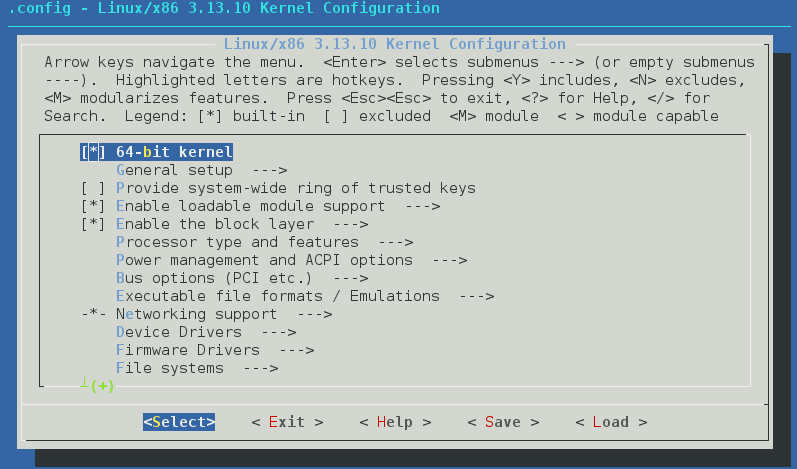
\includegraphics[scale=0.4]{images/menuconfig}
   \end{center}
   \caption[Menuconfig]{Menuconfig}
\end{figure}

Anschliessend wird über \emph{make} der Kernel kompiliert. Für die Installation des Kernels kann
optional auch \emph{make install} ausgeführt werden.

\begin{lstlisting}
$ make
$ sudo make install
\end{lstlisting}

\subsection{Kernel-Modul} \index{Kernel-Modul}

Im Laufe der Entwicklung von Linux sind immer wieder neue Treiber hinzugekommen. Ein Linux-Kernel für einen \keyword{Supercomputer}
benötigt beispielsweise gänzlich andere Treiber als ein \keyword{Embedded-Device}. Um den Kernel je nach Einsatzgebiet anzupassen, werden
Treiber in sogenannten Modulen kompiliert. Module können entweder direkt in das Binary kompiliert werden oder als \keyword{Standalone}.
Über Menuconfig kann dies pro Treiber einzeln festgelegt werden. \\

Das Listing \ref{modul} zeigt ein einfaches \emph{Hello-World}-Modul.
\begin{lstlisting}[label=modul,caption=Hello-World]
#include <linux/module.h>
#include <linux/kernel.h>
#include <linux/init.h>

static int __init helloworld_init (void)
{
        printk(KERN_INFO "hello world\n");
        return 0;
}

static void __exit helloworld_exit (void)
{
        printk(KERN_INFO "good bye world\n");
}

module_init(helloworld_init);
module_exit(helloworld_exit);
\end{lstlisting} \hfill

Sobald das Modul geladen wird, ruft der Kernel die Funktion \emph{helloworld\_init()} auf. Der Rückgabewert Null meldet dem Kernel, dass das Laden erfolgreich war. Bei einem Fehler wird ein Wert ungleich
Null zurückgeben. Im Falle eines dynamischen Moduls wird beim Beenden des Moduls die \emph{helloworld\_exit()} Funktion aufgerufen. 
Mittels \emph{printk()} (print kernel log) kann, analog zum Userspace-Pendant \emph{printf()}, eine Ausgabe gemacht werden.

\subsection{Code-Konvention}

Der Linux-Kernel verwendet einen Standard für die Formatierung des Source-Codes. Es ist zu empfehlen, diesen auch für eigene Treiber anzuwenden,
denn es werden nur Patches mit dieser Konvention akzeptiert. Zudem hilft es auch beim Lesen des restlichen Codes. Der Standard mag auf den ersten
Blick etwas eigenartig wirken. Die Argumente im \emph{Linux Kernel Coding Style} \cite{lkcs} sind jedoch schlüssig:

\begin{itemize}
   \item Der Einzug erfolgt mit Tabs und entspricht acht Spaces. Tabs werden nicht ersetzt.
         Es sollte nie mehr als drei Verschachtlungsebenen geben. Der Code-Guide rechtfertigt dies folgendermassen:
         \enquote{Now, some people will claim that having 8-character indentations makes
            the code move too far to the right, and makes it hard to read on a
            80-character terminal screen.  The answer to that is that if you need
            more than 3 levels of indentation, you're screwed anyway, and should fix
            your program.}

   \item Linien mit mehr als 80 Zeichen werden auf die nächste Zeile gebrochen. Eine Ausnahme gibt es,
         falls der Code dadurch wesentlich schlechter lesbar wird.

   \item Die offene, geschweifte Klammer (\{) folgt direkt dem Ausdruck (Bsp. \emph{if}, \emph{while}), die geschlossene Klammer (\}) steht 
         auf einer eigenen Zeile. Nur bei Funktionen steht die offene Klammer ebenfalls auf einer eigenen Zeile.

   \item Zwischen einem Ausdruck (Bsp. \emph{if}, \emph{while}) und der runden Klammer steht ein Whitespace. Nicht aber bei Funktionsaufrufen (\emph{sizeof(int)}).

   \item Variablen- und Funktionsnamen werden in \emph{Snake-Case}\footnote{\url{https://en.wikipedia.org/wiki/Snake_case}}\index{Snake-Case} geschrieben.
         Auf keinen Fall soll die \emph{ungarische Notation}\footnote{\url{https://en.wikipedia.org/wiki/Hungarian_notation}}\index{Ungarische Notation} verwendet werden:
         \enquote{Encoding the type of a function into the name (so-called Hungarian
            notation) is brain damaged - the compiler knows the types anyway and can
            check those, and it only confuses the programmer.  No wonder MicroSoft
            makes buggy programs.}

   \item Kommentare sollen beschreiben, was der Code macht, nicht wie.
\end{itemize}

Ein einfaches Beispiel zeigt das Listing \ref{codestyle}.
\begin{lstlisting}[label=codestyle,caption=Formatierung des Linux-Kernels]
int main(int argc, char *argv)
{
        switch (argc) {
                case 0: puts("No arguments"); break;
                case 1: puts("One argument"); break;
                default: puts("Multiple arguments"); break;
        }
        return 0;
}
\end{lstlisting}



\subsection{Linux-Entwicklung}

Möchte man Änderungen der Allgemeinheit zur Verfügung stellen, so kann man diese in 
den offziellen Linux-Kernel einbringen. Das Einreichen von Patches erfolgt über die \emph{Linux Kernel Mailing List (LKML)}
\footnote{https://lkml.org}\index{Linux Kernel Mailing List (LKML)}. \\

Als Prozess etabliert hat sich das Modell in Abbildung \ref{fig:linuxdev}. Patches an bestehenden Dateien werden an die Modul-Maintainer, 
neue Module an den Subsystem-Maintainer gerichtet. Anschliessend werden die Patches von unten nach oben weitergereicht. Wird bei einem
Review ein Fehler entdeckt, so ist die Aufgabe des Patch-Antragstellers, diesen zu beheben und neu einzureichen. \\ \newline

\begin{figure}[h!]
   \begin{center}
      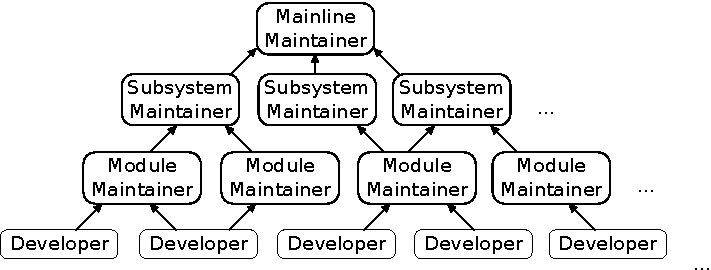
\includegraphics{images/linuxdev}
   \end{center}
   \caption[Linux-Development]{Linux-Development}
   \label{fig:linuxdev}
\end{figure}

\begin{description}[leftmargin=5cm]
   \item[Mainline-Maintainer]
      Welche Patches in den Mainline-Kernel einfliessen ist die Aufgabe von \emph{Linus Torvalds}\index{Linux Torvalds}.
      Er nimmt Patches von Personen entgegen, denen er vertraut. Im Normalfall sind das die Subsystem-Maintainer. Die Diskussion
      findet öffentlich auf der \emph{LKML} statt. 

   \item[Subsystem-Maintainer]
      Als \emph{Subsystem}\index{Subsystem} wird Code bezeichnet, der zwischen mehreren Modulen geteilt wird. Beispiele
      für Subsysteme sind USB, PCI oder Input. Die Subsystem-Maintainer erhalten ihre Patches wiederum von den Modul-Maintainer.

   \item[Modul-Maintainer]
      Um die einzelnen Treiber kümmern sich die Modul-Maintainer. Oft pflegen sie eine ganze Reihe von Modulen. Sie sind
      ein guter Einstiegspunkt um Patches einzureichen.
\end{description}

\subsection{Zusammenfassung}
\begin{itemize}
   \item Sie kennen die Bezugsquellen und die verschiedenen Versionen von Linux
   \item Sie kennen den Aufbau des Source-Codes von Linux
   \item Sie kennen den Buildprozess des Linux-Kernels
   \item Sie kennen den modularen Aufbau von Linux
   \item Sie kennen die Code-Konventionen von Linux
   \item Sie kennen den Entwicklungsprozess von Linux
\end{itemize}

\summary{
Der Linux-Kernel kann über \url{https://kernel.org} bezogen werden. 
Es werden verschiedene Entwicklungsstände angeboten: Mainline, Stable und Longterm. \hfill \\

Wichtige Ordner im Source-Code sind: die Dokumentation (/Documentation), die Treiber (/drivers), Filesysteme (/fs), die
Initialisierung (/init), der Kern (/kernel), die Speicherverwaltung (/mm) und der Netzwerkstack (/net). \hfill \\

Der Kernel wird über \emph{make menuconfig} konfiguriert und mit \emph{make} wird der Build erstellt. \hfill \\

Treiber werden in sogenannten Modulen entwickelt. \hfill \\

Der Entwicklungsprozess findet zwischen den Maintainern auf der \emph{LKML} statt.
}

\subsection{Diskussion}

\begin{itemize}
   \item Welche Versionsbezeichung beinhaltet die neusten Patches? 
   \item Wo würden Sie im Source-Code nach dem USB-Mouse-Treiber suchen?
   \item Ist es möglich den Linux-Kernel ohne Netzwerk-Stack zu bauen?
   \item Was ist der Vor-/Nachteil, wenn Module direkt in den Kernel kompiliert werden?
   \item Ist der Linux-Kernel wegen des Supports von Modulen noch ein \emph{monolithischer Kernel}\index{Monolithischer Kernel}? 
         Oder eher ein \emph{Mikrokernel}\index{Mikrokernel}? Wieso?
\end{itemize}
